\documentclass[
    ngerman,
    color=3b,
    dark_mode,
    % load_common, % Loads a list of commonly used Packages
    summary,
    boxarc,
    % manual_term,
    % solution=true,
]{rubos-tuda-template} 
% Import all Packages from Main Preamble with relative Path
% \subimport*{../../}{preamble}
% Get Labels from Main Document using the xr-hyper Package
\externaldocument[ext:]{../../AuD-Zusammenfassung-2020}
% Set Graphics Path, so pictures load correctly
\graphicspath{{../../}}

\usetag{full}

\begin{document}

\section{Sortieren}\label{2}\label{Sortieren}\index{Sortieren}
\subsection{Einführung - Das Sortierproblem}\label{2.1}\label{Einfuehrung Sortieren}\index{Sortierproblem}
% \paragraph{Problemstellung:}
\begin{definition}[Das Sortierproblem]\mbox{}\\
    \fatsf{Ausgangspunkt}:
    \begin{center}
        \captionsetup{type=figure}
        \includestandalone[width=.2\textwidth]{pictures/folge_von_Datensaetzen/folge_von_Datensaetzen}% 
        \captionof{figure}{Folge von Datensätzen $D_1,D_2,\cdots,D_n$}
        \label{fig:folge_von_Datensätzen}
    \end{center}

    \fatsf{Ziel}:  Datensätze so anzuordnen, dass die Schlüsselwerte sukzessive
    ansteigen (oder absteigen)\\
    \fatsf{Bedingung}: Schlüssel(werte) müssen vergleichbar sein
\end{definition}
\begin{itemize}
    \item zu sortierende Elemente hei\ss{}en auch Schlüssel(werte)
\end{itemize}
\begin{grayInfoBox}[title=Durchführung]
    \begin{itemize}
        \item \fatsf{Eingabe}: Sequenz von Schlüsselwerten $\left\{a_1,a_2,\ldots,a_n\right\}$
        \item Eingabe ist eine \fatsf{Instanz} des Sortierproblems
        \item \fatsf{Ausgabe}: Permutation $\left\{a_1',a_2',\ldots,a_n'\right\}$ derselben Folge mit Eigenschaft $a_1'\leq\ldots\leq a_n'$
        \item Algorithmus ist \fatsf{korrekt}, wenn dieser das Problem für alle Instanzen löst
    \end{itemize}
\end{grayInfoBox}
\subsection{Arrays}\label{2.2}\label{Arrays}\index{Array}
\begin{definition}[Array]
    Reihung (Feld) fester Länge von Daten des gleichen Typs
\end{definition}
\begin{figure}[h]
    \centering
    \includestandalone[]{pictures/array_beispiel/array_beispiel}% 
    \caption{beispielhafte Darstellung eines Arrays}
    \label{fig:array_beispiel}
\end{figure}
\begin{description}[leftmargin=1cm]
    \item [$A$] Bezeichnung des Arrays mit dem Namen "`$A$"'
    \item [{$A[i]$}] Zugiff auf das $(i+1)$-te Element des Arrays
\end{description}
\paragraph{Beispiel:}\mbox{}
\begin{grayInfoBox}
    $A[2]=17$
\end{grayInfoBox}
$\Longrightarrow$ Arrays erlauben effizienten Zugriff auf Elemente: konstanter Aufwand
\clearpage
\subsection{Exkurs: Totale Ordnung}\label{Totale Ordnung}\index{Totale Ordnung}
\begin{definition}[Totale Ordnung]
    Sei $M$ eine nicht leere Menge und $\leq \subseteq M\times M $ eine binäre Relation auf $M$.

    Das Paar $(M,\leq)$ hei\ss{}t genau dann eine totale Relation auf der Menge $M$, wenn folgende Eigenschaften erfüllt sind:
    \begin{itemize}
        \item Reflexivität\index{Reflexivität}: $\forall x \in M: x \leq x$
        \item Transitivität\index{Transitivität}: $\forall x,y,z\in M: x\leq y \land y \leq z \Rightarrow x \leq z$
        \item Antisymmetrie\index{Antisymmetrie}: $\forall x,y\in M: x\leq y \land y \leq x \Rightarrow x = y$
        \item Totalität\index{Totalität}: $\forall x,y \in M : x\leq y \lor y \leq x$
    \end{itemize}
\end{definition}
\paragraph{Beispiele}\mbox{}
\begin{grayInfoBox}
    \begin{itemize}
        \item $\leq$ Ordnung auf natürlichen Zahlen
        \item Lexikographische Ordnung $\leq_{lex}$ ist eine totale Ordnung
    \end{itemize}
\end{grayInfoBox}
\subsection{Vergleichskriterien von Suchalgorithmen}\label{Vergleichskriterien von Suchalgorithmen}
\begin{description}[leftmargin=3.6cm,itemsep=1em]
    \item[Berechnungsaufwand] \begin{itemize}
            \item $\mathcal{O}(n)$
        \end{itemize}
    \item[Effizienz] \begin{itemize}
            \item Best Case vs. Average Case vs Worst Case
        \end{itemize}
    \item[Speicherbedarf] \begin{itemize}
            \item in-Place (in situ): zusätzlicher Speicher von der Eingabegrö\ss{}e unabhängig
            \item out-of-place: Speichermehrbedarf von Eingabegrö\ss{}e abhängig
        \end{itemize}
    \item[Stabilität] \begin{itemize}
            \item stabile Verfahren verändern die Reihenfolge von äquivalenten Elementen nicht
        \end{itemize}
    \item[Anwendung als Auswahlfaktor] \begin{itemize}
            \item Hauptoperationen beim Sortieren: Vergleichen und Vertauschen
            \item Anwendung spielt eine enorme Rolle:\begin{itemize}
                      \item Verfahren mit vielen Vertauschungen und wenig Vergleichen, wenn Vergleichen teuer
                      \item Verfahren mit wenig Vertauschungen und vielen Vergleichen, wenn Umsortieren teuer
                  \end{itemize}
        \end{itemize}
\end{description}
\clearpage
\subsection{Analyse von Algorithmen \textmd{(I)}}\label{Analyse von Algorithmen 1}
\paragraph{Schleifeninvariante \textmd{(SIV)}:}\index{Schleifeninvariante}
\begin{itemize}
    \item Sonderform der Invariante
    \item Am Anfang/Ende jedes Schleifendurchlaufs und vor/nach jedem Schleifendurchlauf gültig
    \item Wird zur Feststellung der Korrektheit von Algorithmen verwendet
    \item Eigenschaften:
          \begin{description}
              \item [Initialisierung] Invariante ist vor jeder Iteration wahr
              \item [Fortsetzung] Wenn SIV vor der Schleife wahr ist, dann auch bis Beginn der nächsten Iteration
              \item [Terminierung] SIV liefert bei Schleifenabbruch, helfende Eigenschaft für Korrektheit
          \end{description}
    \item Beispiel für Umsetzung: \hyperref[insSortSiv]{\textcolor{red}{Insertion Sort - SIV}}
\end{itemize}

\paragraph{Laufzeitanalyse:}\index{Laufzeitanalyse}
\begin{itemize}
    \item Aufstellung der Kosten und Durchführungsanzahl für jede Zeile des Quelltextes
    \item Beachte: Bei Schleifen wird auch der Aufruf gezählt, der den Abbruch einleitet
    \item Beispiel für Umsetzung: \hyperref[insSortLaufzeit]{\textcolor{red}{Insertion Sort - Laufzeit}}
    \item Zusätzliche Überprüfung des \texttt{Best Case, Worst Case} und \texttt{Average Case}
\end{itemize}

\paragraph{Effizienz von Algorithmen:}\index{Effizienz von Algorithmen}
\begin{description}[leftmargin=7cm,itemsep=1em]
    \item [Effizienzfaktoren]
          \begin{itemize}
              \item Rechenzeit (Anzahl der Einzelschritte)
              \item Kommunikationsaufwand
              \item Speicherplatzbedarf
              \item Zugriffe auf Speicher
          \end{itemize}
    \item [Laufzeitfaktoren]
          \begin{itemize}
              \item Länge der Eingabe
              \item Implementierung der Basisoperationen
              \item Takt der CPU
          \end{itemize}
\end{description}
\clearpage
\subsection{Analyse von Algorithmen \textmd{(II)}}\label{Analyse von Algorithmen 2}
\paragraph{Komplexität:}\index{Komplexität}
\begin{itemize}
    \item Abstrakte Rechenzeit $T(n)$ ist abhängig von den Eingabedaten
    \item Übliche Betrachtungsweise der Rechenzeit ist asymptotische Betrachtung
\end{itemize}

\paragraph{Asymptotik:}\index{Asymptotik}
\begin{itemize}
    \item Annäherung an einer sich ins Unendliche verlaufende Kurve
    \item z.B.: $f(x) = \frac{1}{x} + x$ | Asymptote: $g(x)=x$ | ($\frac{1}{x}$ läuft gegen Null)
\end{itemize}

\paragraph{Asymptotische Komplexität:}\index{Asymptotische Komplexität}
\begin{itemize}
    \item Abschätzung des zeitlichen Aufwands eines Algorithmus in Abhängigkeit einer Eingabe
    \item Beispiel für Umsetzung: \hyperref[insSortLaufzeitTheta]{\textcolor{red}{Insertion Sort - Laufzeit $\Theta$}}
\end{itemize}

\paragraph{Asymptotische Notation:}\index{Asymptotische Notation}
\begin{itemize}
    \item Betrachtung der Laufzeit $T(n)$ für sehr gro\ss e Eingaben $n \in \mathbb{N}$
    \item Komplexität ist unabhängig von konstanten Faktoren und Summanden
    \item Nicht berücksichtigt: Rechnergeschwindigkeit / Initialisierungsaufwände
    \item Komplexitätsmessung via Funktionsklasse ausreichend
          \begin{itemize}
              \item Verhalten des Algorithmus für gro\ss e Problemgrö\ss en
              \item Veränderung der Laufzeit bei Verdopplung der Problemgrö\ss e
          \end{itemize}
\end{itemize}

\paragraph{Gründe für die Nutzung der theoretischen Betrachtung statt der Messung der Laufzeit }
\begin{description}[itemsep=1em]
    \item [Vergleichbarkeit]
          \begin{itemize}
              \item Laufzeit abhängig von konkreter Implementierung und System
              \item Theoretische Betrachung ist frei von Abhängigkeiten und Seiteneffekten
              \item Theoretische Betrachtung lässt direkte Vergleichbarkeit zu
          \end{itemize}

    \item [Aufwand]
          \begin{itemize}
              \item Wieviele Testreihen?
              \item In welcher Umgebung?
              \item Messen führt in der Ausführung zu hohem, praktischen Aufwand
          \end{itemize}

    \item [Komplexitätsfunktion]
          \begin{itemize}
              \item Wachstumsverhalten ausreichend
              \item Praktische Evaluation mit Zeiten nur für Auswahl von Systemen möglich
              \item Theoretischer Vergleich (Funktionsklassen) hat ähnlichen Erkenntnisgewinn
          \end{itemize}
\end{description}
\clearpage
\subsection{Analyse von Algorithmen \textmd{(III)}}\label{Analyse von Algorithmen 3}
\paragraph{Übersicht}\mbox{}
\begin{description}[leftmargin=2cm]
    \item [$\Theta$] $=$
    \item [$\mathcal{O}$] $\leq$
    \item [$\Omega$] $\geq$
\end{description}
\paragraph{$\Theta$-Notation}\index{$\Theta$-Notation}
\begin{wrapfigure}[5]{r}{.3\textwidth}
    \centering
    \includegraphics[width=5cm]{pictures/thetaNotationGraph\IfDarkModeT{_dark}.pdf}
    \caption{Veranschaulichung $\Theta$-Notation}
    \label{fig:theta_notation}
\end{wrapfigure}
\begin{itemize}
    \item $\Theta$-Notation beschränkt eine Funktion asymptotisch von oben und unten
    \item Funktionen $f,g: \mathbb{N} \rightarrow \mathbb{R}_{>0}$ ($\mathbb{N}$: Eingabelänge, $\mathbb{R}$: Zeit)
    \item[] \includegraphics[width=\linewidth]{pictures/thetaNotation\IfDarkModeT{_dark}.pdf}
    \item $\Theta(g)$ enthält alle $f$, die genauso schnell wachsen wie $g$
    \item \fatsf{Schreibweise}: $f \in \Theta(g)$ (korrekt), manchmal auch $f = \Theta(g)$

    \item $g(n)$ ist eine asymptotisch scharfe Schranke von $f(n)$
    \item $f(n)= \Theta(g(n))$ gilt, wenn $f(n) = O(g(n))$ und $f(n)=\Omega(g(n))$ erfüllt sind
    \item z.B.: $f(n)= \frac{1}{2} n^2 - 3n$ | $f(n) \in \Theta(n^2)$?
    \item Aus $\Theta(n^2)$ folgt, dass $g(n)=n^2$
    \item \fatsf{Vorgehen}:
          \begin{itemize}
              \item Finden eines $n_0$ und $c_1,c_2$, sodass
              \item $c_1*g(n) \leq f(n) \leq c_2*g(n)$ erfüllt ist
              \item Konkret: $c_1*n^2 \leq \frac{1}{2} n^2 - 3n \leq c_2*n^2$
              \item Division durch $n^2$: $c_1 \leq \frac{1}{2}-\frac{3}{n} \leq c2$
              \item Ab $n=7$ positives Ergebnis: $0,0714$ | $n_0 = 7$
              \item Deswegen setzen wir $c_1=\frac{1}{14}$
              \item Für $n \rightarrow \infty: ~ 0,5$ | $c_2 = 0,5$
              \item Natürlich auch andere Konstanten möglich
          \end{itemize}
\end{itemize}


\pagebreak

\paragraph{$\mathcal{O}$-Notation}\index{$\mathcal{O}$-Notation}
\begin{wrapfigure}[5]{r}{.3\textwidth}
    \centering
    \includegraphics[width=5cm]{pictures/oNotationGraph\IfDarkModeT{_dark}.pdf}
    \caption{Veranschaulichung $\mathcal{O}$-Notation}
    \label{fig:o-notation}
\end{wrapfigure}
\begin{itemize}
    \item $\mathcal{O}$-Notation beschränkt eine Funktion asymptotisch von oben
    \item[] \includegraphics[width=\linewidth]{pictures/oNotation\IfDarkModeT{_dark}.pdf}
    \item $O(g)$ enthält alle $f$, die höchstens so schnell wie $g$ wachsen
    \item \fatsf{Schreibweise}: $f=\mathcal{O}(g)$
    \item $f(n)=\Theta(g) \rightarrow f(n) = \mathcal{O}(g)$ | $\Theta(g(n)) \subseteq \mathcal{O}(g(n))$
    \item Ist $f$ in der Menge $\Theta(g)$, dann auch in der Menge $\mathcal{O}(g)$
    \item z.B.: $f(n) = n + 2$ | $f(n) = \mathcal{O}(n)$?
    \item Ja $f(n)$ ist Teil von $\mathcal{O}(n)$ für z.B. $c = 2$ und $n_0 = 2$
\end{itemize}

\paragraph{$O$-Notation Rechenregeln}
\begin{description}[itemsep=1em]
    \item [Konstanten]
          \begin{itemize}
              \item $f(n) = a$ mit $a \in \mathbb{R}$ konstante Funktion $\rightarrow$ $f(n) = O(1)$
              \item z.B. $3 \in O(1)$
          \end{itemize}

    \item [Skalare Multiplikation]
          \begin{itemize}
              \item $f= O(g)$ und $a \in \mathbb{R}$ $\rightarrow$ $a*f = O(g)$
          \end{itemize}

    \item [Addition]
          \begin{itemize}
              \item $f_1 = O(g_1)$ und $f_2 = O(g_2)$ $\rightarrow$ $f_1+f_2= O(max\{g_1,g_2\})$
          \end{itemize}

    \item [Multiplikation]
          \begin{itemize}
              \item $f_1 = O(g_1)$ und $f_1 = O(g_2)$ $\rightarrow$ $f_1*f_2= O(g_1*g_2)$
          \end{itemize}
\end{description}

\paragraph{$\Omega$-Notation}\index{$\Omega$-Notation}
\begin{wrapfigure}[5]{r}{.3\textwidth}
    \centering
    \includegraphics[width=5cm]{pictures/omegaNotationGraph\IfDarkModeT{_dark}.pdf}
    \caption{Veranschaulichung}
    \label{fig:omega-notation}
\end{wrapfigure}
\begin{itemize}
    \item $\Omega$-Notation beschränkt eine Funktion asymptotisch von unten
    \item[] \includegraphics[width=\linewidth]{pictures/omegaNotation\IfDarkModeT{_dark}.pdf}
    \item $\Omega$-Notation enthält alle $f$, die mindestens so schnell wie $g$ wachsen
    \item \fatsf{Schreibweise}: $f = \Omega(g)$
\end{itemize}
\clearpage
\paragraph{Komplexitätsklassen}\index{Komplexitätsklassen}\mbox{}

\begin{table}[ht]
    \centering
    \rowcolors{2}{\thepagecolor}{fgcolor!10!\thepagecolor}
    \renewcommand{\arraystretch}{1.2}
    \begin{tabular}{cll}
        \toprule
        Klasse            & Bezeichnung   & Beispiel               \\
        \midrule
        $\Theta(1)$       & Konstant      & Einzeloperation        \\
        $\Theta(\log n)$  & Logarithmisch & Binäre Suche           \\
        $\Theta(n)$       & Linear        & Sequentielle Suche     \\
        $\Theta(n\log n)$ & Quasilinear   & Sortieren eines Arrays \\
        $\Theta(n^2)$     & Quadratisch   & Matrixaddition         \\
        $\Theta(n^3)$     & Kubisch       & Matrixmultiplikation   \\
        $\Theta(n^k)$     & Polynomiell   &                        \\
        $\Theta(2^n)$     & Exponentiell  & Travelling-Salesman*   \\
        $\Theta(n!)$      & Faktoriell    & Permutationen          \\
        \bottomrule
    \end{tabular}
    \caption{Komplexitätsklassen ($n$= Länge der Eingabe)}
    \label{tab:komplexitaetsklassen}
\end{table}
% \item[] 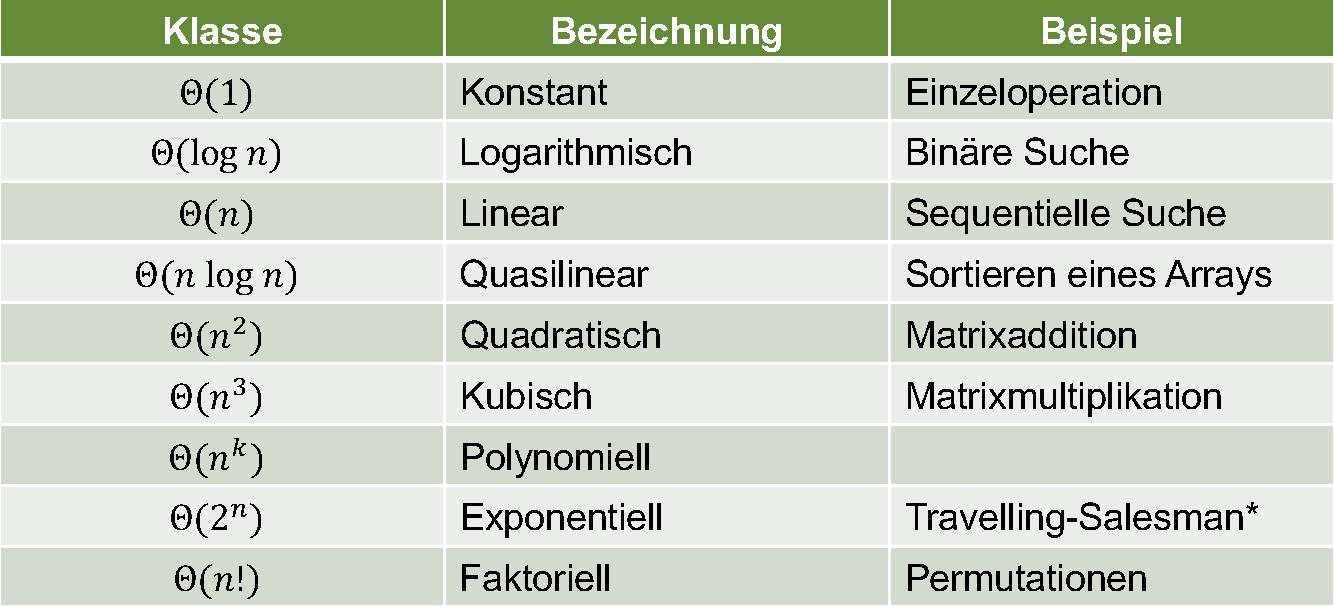
\includegraphics[width=12cm]{pictures/komplexitaetsklassen.pdf}
\begin{table}[ht]
    \centering
    \rowcolors{2}{\thepagecolor}{fgcolor!10!\thepagecolor}
    \renewcommand{\arraystretch}{1.2}
    \begin{tabular}{cccccc}
        \toprule
        Eingabegrö\ss{}e $n$ & $\log_{10} n$     & $n$                 & $n^2$                                     & $n^3$                         & $2^n$                             \\
        \midrule
        10                   & $1\mathrm{\mu s}$ & $10\mathrm{\mu s}$  & $100\mathrm{\mu s}$                       & $1\mathrm{ms}$                & $\sim 1~\mathrm{ms}$              \\
        100                  & $2\mathrm{\mu s}$ & $100\mathrm{\mu s}$ & $10\mathrm{ms}$                           & $1\mathrm{s}$                 & $\sim 4\times 10^{16}~\mathrm{y}$ \\
        1000                 & $3\mathrm{\mu s}$ & $1\mathrm{ms}$      & $1s$                                      & $16\mathrm{min}~40\mathrm{s}$ & $?$                               \\
        10000                & $4\mathrm{\mu s}$ & $10\mathrm{ms}$     & $1\mathrm{min}~40\mathrm{s}$              & $\sim 11,5\mathrm{d}$         & $?$                               \\
        100000               & $5\mathrm{\mu s}$ & $100\mathrm{ms}$    & $2\mathrm{h}~64\mathrm{min}~40\mathrm{s}$ & $\sim 31,7\mathrm{y}$         & $?$                               \\
        \bottomrule
    \end{tabular}
    \caption{Komplexitätsklassen-Ausführungsdauer, falls eine Operation $n$ genau $1\mu s$ dauert}
    \label{tab:komplexitaetsklassen-Ausfuehrungezeit}
\end{table}
% \item[] 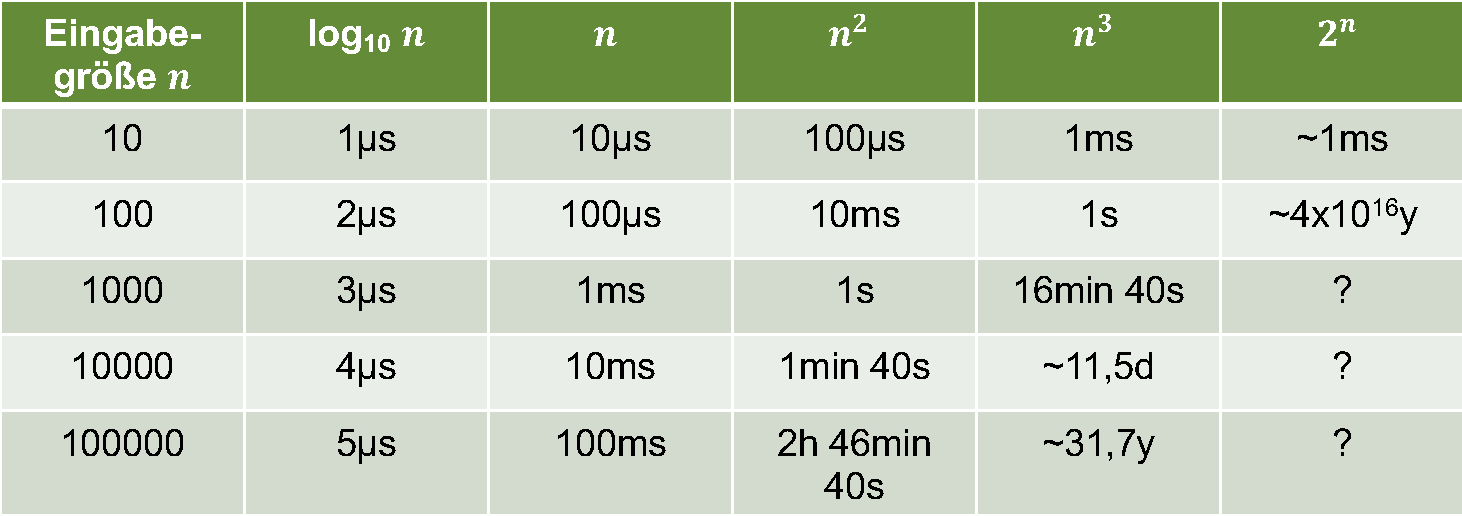
\includegraphics[width=12cm]{pictures/komplexitaetsklassenDauer.pdf}

Es gilt: $\log(n) < \sqrt{n} < n < n\cdot \log(n) < n^2 < n! < 2^n<n^n$
\vspace*{-2ex}
\paragraph{Asymptotische Notationen in Gleichungen}
\begin{itemize}
    \item $2n^2 + 3n + 1 = 2n^2 + \Theta(n)$
    \item $\Theta(n)$ fungiert hier als Platzhalter für eine beliebige Funktion $f(n)$ aus $\Theta(n)$
    \item z.B.: $f(n) = 3n + 1$
\end{itemize}
\vspace*{-2ex}
\paragraph{$o$-Notation}
\begin{itemize}
    \item $o$-Notation stellt eine echte obere Schranke dar
    \item Ausschlaggebend ist, dass es für alle $c \in \mathbb{R}_{>0}$ gelten muss
    \item Au\ss erdem $<$ statt $\leq$
    \item z.B.: $2n = o(n^2)$ und $2n^2 \neq o(n^2)$
    \item[] %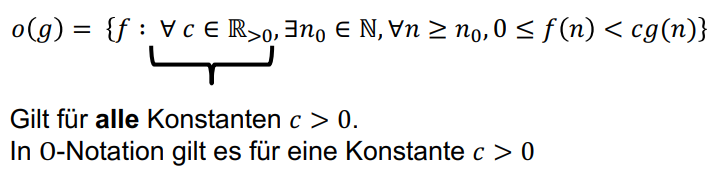
\includegraphics[width=12cm]{pictures/oKleinNotation.PNG}
        $o(g)=\{f:\underbrace{\forall c \in \mathbb{R}_{>0}}_{
            \mathclap{
                \substack{
                    \text{Gilt für \fatsf{alle} Konstanten $c>0$.}\\
                    \text{In $\mathcal{O}$-Notation gilt es für eine Konstante $c>0$}}}
            }, \exists n_0 \in \mathbb{N}, \forall n \geq n_0, 0\leq f(n)<cg(n)\}$
\end{itemize}

\paragraph{$\omega$-Notation}
\begin{itemize}
    \item $\omega$-Notation stellt eine echte untere Schranke dar
    \item Ausschlaggebend ist, dass es für alle $c \in \mathbb{R}{>0}$ gelten muss
    \item Au\ss erdem $>$ statt $\geq$
    \item z.B.: $\frac{n^2}{2} = \omega(n)$ und $\frac{n^2}{2} \neq \omega(n^2)$
    \item[] %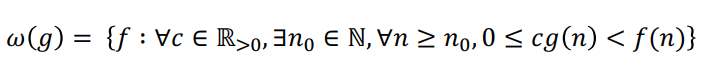
\includegraphics[width=12cm]{pictures/omegaKleinNotation.PNG}
        $\omega(g)=\{f:\forall c \in \mathbb{R}_{>0},\exists n_0 \in \mathbb{N} \forall n \geq n_0,0\leq cg(n)<f(n)\}$
\end{itemize}
\clearpage
\subsection{Insertion Sort \textmd{(Sortieren durch Einfügen)}}\label{InsertionSort}\index{Insertion Sort}
\begin{idea}[Insertion-Sort]\mbox{}
    \begin{itemize}
        \item Halte die linke Teilfolge sortiert
        \item Füge nächsten Schlüsselwert hinzu, indem es an die korrekte Position eingefügt wird
        \item Wiederhole den Vorgang bis Teilfolge aus der gesamten Liste besteht
    \end{itemize}
\end{idea}
\paragraph{Code}\mbox{}
%\begin{noindent}
\begin{codeBlock}[autogobble]{title=Insertion-Sort(A)}
    FOR j = 1 TO A.length - 1
      key = A[j]
      // Füge A[j] in die sortierte Sequenz A[0...j-1] ein
      i = j - 1
      WHILE i >= 0 and A[i] > key
          A[i + 1] = A[i]
          i = i - 1
      A[i + 1] = key
\end{codeBlock}
%\end{noindent}

\paragraph{Schleifeninvariante von \texttt{Insertion Sort}}\label{insSortSiv}
\begin{itemize}
    \item Zu Beginn jeder Iteration der \texttt{for}-Schleife besteht die Teilfolge \texttt{A[0...j-1]} aus den Elementen \\
          der ursprünglichen Teilfolge \texttt{A[0...j-1]} enthaltenen Elementen, allerdings in sortierter Reihenfolge.
\end{itemize}

\paragraph{Korrektheit von \texttt{Insertion Sort}}
\begin{description}[leftmargin=3cm,itemsep=1em]
    \item [Initialisierung]
          Beginn mit \texttt{j=1}, also Teilfeld \texttt{A[0...j-1]} besteht nur aus einem Element \texttt{A[0]}. \\
          Dies ist auch das ursprüngliche Element und Teilfeld ist sortiert.
    \item [Fortsetzung]
          Zu zeigen ist, dass die Invariante bei jeder Iteration erhalten bleibt. Ausführungsblock der \texttt{for}-Schleife
          sorgt dafür, dass \texttt{A[j-1], A[j-2]},... je um Stelle nach rechts geschoben werden bis \texttt{A[j]} korrekt eingefügt wurde.
          Teilfeld \texttt{A[0...j]} besteht aus ursprünglichen Elementen und ist sortiert. Inkrementieren von j erhält die Invariante.
    \item [Terminierung]
          Abbruchbedingung der \texttt{for}-Schleife, wenn \texttt{j > A.length - 1}. Jede Iteration erhöht j.
          Dann bei Abbruch ist \texttt{j = n } und einsetzen in Invariante liefert das Teilfeld \texttt{A[0...n-1]}
          welches aus den ursprünglichen Elementen besteht und sortiert ist. Teilfeld ist gesamtes Feld.
\end{description}
$\Longrightarrow$ Algorithmus \texttt{Insertion Sort} arbeitet damit korrekt.
\clearpage
\paragraph{Laufzeitanalyse von \texttt{Insertion Sort}} {\label{insSortLaufzeit}}\mbox{}
\vspace*{1em}\\
\begin{minipage}[c]{0.3\textwidth}
    \mbox{}
    \centering
    % \renewcommand{\arraystretch}{.8}
    % \rowcolors{2}{white}{black!10}
    \resetrc
    \resizebox{\textwidth}{!}{%
        \begin{tabular}{ccc}
            \toprule
            \fatsf{Zeile} & \fatsf{Kosten} & \fatsf{Anzahl}                         \\
            \midrule
            1             & $c_1$          & $n$                                    \\
            2             & $c_2$          & $n-1$                                  \\
            3             & $0$            & $n-1$                                  \\
            4             & $c_4$          & $n-1$                                  \\
            5             & $c_5$          & $\displaystyle\sum_{j=1}^{n-1}t_j$     \\
            6             & $c_6$          & $\displaystyle\sum_{j=1}^{n-1}(t_j-1)$ \\
            7             & $c_7$          & $\displaystyle\sum_{j=1}^{n-1}(t_j-1)$ \\
            8             & $c_8$          & $n-1$                                  \\
            \bottomrule
        \end{tabular}}
    %\caption{Laufzeitanalyse von Insertion-Sort}
    \label{tab:insertion-sort:laufzeit}
\end{minipage}
\begin{minipage}[c]{0.6\textwidth}
    \begin{itemize}
        \item Festlegung der Laufzeit für jede Zeile
        \item Jede Zeile besitzt gewissen Kosten \texttt{$c_i$}
        \item Jede Zeile wird $x$ mal durchgeführt
        \item $Laufzeit = Anzahl * Kosten$ jeder Zeile
        \item Schleifen: Abbruchüberprüfung zählt auch
        \item \texttt{$t_j$}: Anzahl der Abfragen der \texttt{While}-Schleife
        \item Laufzeit:
              $T(n)=c_{1} n+c_{2}(n-1)+c_{4}(n-1)+c_{5} \sum_{j=1}^{n-1} t_{j}\\ +c_{6} \sum_{j=1}^{n-1}\left(t_{j}-1\right)+c_{7} \sum_{j=1}^{n-1}\left(t_{j}-1\right)+c_{8}(n-1)$
    \end{itemize}
\end{minipage}
% \vspace{1em}
\begin{description}[itemsep=1em]
    \item [Warum $n$ in Zeile 1?]
          \begin{itemize}
              \item Die Überprüfung der Fortführungsbedingung beinhaltet auch die letze Überprüfung
              \item Quasi die Überprüfung, durch die die Schleife abbricht
          \end{itemize}

    \item [Warum $\sum^{n-1}_{j=1}$ in Zeile 5?]
          \begin{itemize}
              \item Aufsummierung aller einzelnen $t_j$ über die Anzahl der Schleifendurchläufe
              \item Diese ist allerdings $n-1$ und nicht $n$, da die Abbruchüberprüfung dort auch enthalten ist
          \end{itemize}

    \item [Warum $t_j-1$ in Zeile 6?]
          \begin{itemize}
              \item Selbes Argument wie oben, bei $t_j$ ist die Abbruchüberprüfung enthalten
              \item Deswegen wird die \texttt{while}-Schleife nur $t_j-1$-mal ausgeführt
          \end{itemize}

    \item [\texttt{Best Case}]
          \begin{itemize}
              \item zu sortierendes Feld ist bereits sortiert
              \item $t_j$ wird dadurch zu 1, da die \texttt{While}-Schleife immer nur einmal prüft (Abbruch)
              \item Die zwei Zeilen innerhalb der \texttt{While}-Schleife werden nie ausgeführt
              \item Durch Umformen ergibt sich, dass die Laufzeit eine lineare Funktion in $n$ ist
          \end{itemize}

    \item [\texttt{Worst Case}]
          \begin{itemize}
              \item zu sortierendes Feld ist umgekehrt sortiert
              \item $t_j$ wird dadurch zu $j+1$, da die \texttt{While}-Schleife immer die gesamte Länge prüft
              \item Durch Umformen ergibt sich, dass die Laufzeit eine quadratische Funktion in $n$ ist ($n^2$)
          \end{itemize}

    \item [\texttt{Average Case}]
          \begin{itemize}
              \item im Mittel gut gemischt
              \item $t_j$ wird dadurch zu $j/2$
              \item Die Laufzeit bleibt aber eine quadratische Funktion in $n$ ($n^2$)
          \end{itemize}
\end{description}

\paragraph{Asymptotische Laufzeitbetrachtung $\Theta$} {\label{insSortLaufzeitTheta}}
\begin{itemize}
    \item $T(n)$ lässt sich als quadratische Funktion $an^2 + bn + c$ betrachten
    \item Terme niedriger Ordnung sind für gro\ss e $n$ irrelevant
    \item Deswegen Vereinfachung zu $n^2$ und damit $\Theta(n^2)$
\end{itemize}
\clearpage
\begin{taggedblock}{KW,full}
    \subsection{String matching}\label{StringMatching}\index{String Matching}
    \begin{idea}[String matching]\mbox{}
        \begin{itemize}
            \item Gegeben: String $S$, Suchstring $T$, Alphabet $A$
            \item Ziel: Finde alle Vorkommen von $T$ in $S$ ohne Duplikate (aufsteigend Sortiert)
        \end{itemize}
    \end{idea}

    \subsubsection{Iterativ}
    \paragraph{Code}\mbox{}

    %\begin{noindent}
    \begin{codeBlock}[autogobble]{title={StringMatching(S,T,A)}}
        IF S.length < T.length
            return [];                // No Match possible
        I=[]
        R=[]
        FOR i = 0 TO S.length
            FOR j = 0 TO I.length - 1
                IF S[i] != T[i-I[j]]
                    I.remove(I[j]);   // Valid Candidate
                IF i-I[j] == T.length
                    R.add[I[j]];      // Match Found
            IF S[i] == T[0]
                I.add(i);
        return R;
    \end{codeBlock}
    %\end{noindent}
    \paragraph{Analyse von \texttt{String matching}}
    \begin{description}[leftmargin=5cm,itemsep=1em]
        \item [Komplexität]
              \begin{itemize}
                  %   \item \texttt{Best Case}: $\Theta(n)$
                  %   \item \texttt{Average Case}: $\Theta(n^2)$
                  \item \texttt{Worst Case}: $\mathcal{O}(\vert S\vert\cdot\vert T\vert)$.
              \end{itemize}
    \end{description}
    \subsubsection{Als Endlicher automat}\label{BOFAStringMatching}\index{BOFA String Matching}
    \begin{figure}[h]
        \centering
        \includestandalone[]{pictures/string-matching_bofa/string-matching_bofa}
    \end{figure}
    \clearpage
\end{taggedblock}
%
\subsection{Bubble Sort}\label{BubbleSort}\index{Bubble Sort}
\begin{idea}[Bubble Sort]\mbox{}
    \begin{itemize}
        \item Vergleiche Paare von benachbarten Schlüsselwerten
        \item Tausche das Paar, falls rechter Schlüsselwert kleiner als linker
    \end{itemize}
\end{idea}

\paragraph{Code}\mbox{}
%\begin{noindent}
\begin{codeBlock}[autogobble]{title=BubbleSort(A)}
    FOR i = 0 TO A.length - 2
        FOR j = A.length - 1 DOWNTO i + 1
            IF A[j] < A[j-1]
                SWAP(A[j], A[j-1])
\end{codeBlock}
%\end{noindent}

\paragraph{Analyse von \texttt{Bubble Sort}}
\begin{description}[leftmargin=5cm,itemsep=1em]
    \item [Anzahl der Vergleiche]
          \begin{itemize}
              \item Es werden stets alle Elemente der Teilfolge miteinander verglichen
              \item Unabhängig von der Vorsortierung sind \texttt{Worst} und \texttt{Best Case} identisch
          \end{itemize}

    \item [Anzahl der Vertauschungen]
          \begin{itemize}
              \item \texttt{Best Case}: 0 Vertauschungen
              \item \texttt{Worst Case}: $\dfrac{n^2-n}{2}$ Vertauschungen
          \end{itemize}

    \item [Komplexität]
          \begin{itemize}
              \item \texttt{Best Case}: $\Theta(n)$
              \item \texttt{Average Case}: $\Theta(n^2)$
              \item \texttt{Worst Case}: $\Theta(n^2)$
          \end{itemize}
\end{description}

% \clearpage
\subsection{Selection Sort}\label{Selection sort}\index{Selection Sort}
\begin{idea}[Selection Sort]
    \begin{itemize}
        \item Sortieren durch direktes Auswählen
        \item \texttt{MinSort}\index{MinSort}: "wähle kleines Element in Array und tausche es nach vorne"
        \item \texttt{MaxSort}\index{MaxSort}: "wähle grö\ss{}tes Element in Array und tausche es nach vorne"
    \end{itemize}
\end{idea}

\paragraph{Code} (MinSort)
%\begin{noindent}
\begin{codeBlock}[autogobble]{title=Selection-Sort(A)}
    FOR i = 0 TO A.length - 2
        k = i
        FOR j = i + 1 TO A.length - 1
            IF A[j] < A[k]
                k = j
        SWAP(A[i], A[k])
\end{codeBlock}
%\end{noindent}

\clearpage
\subsection{Divide-And-Conquer Prinzip}\label{Divide-And-Conquer}\index{Divide-And-Conquer}
\begin{idea}[Divide-And-Conquer]\mbox{}\\
    Zerlege das Problem und löse es direkt oder zerlege es weiter:
    \begin{description}[leftmargin=2cm,itemsep=1em]
        \item [Divide]\index{Divide}
              \begin{itemize}
                  \item Teile das Problem in mehrere Teilprobleme auf
                  \item Teilprobleme sind Instanzen des gleichen Problems
              \end{itemize}
        \item [Conquer]\index{Conquer}
              \begin{itemize}
                  \item Beherrsche die Teilprobleme rekursiv
                  \item Falls Teilprobleme klein genug, löse sie auf direktem Weg
              \end{itemize}
        \item [Combine]\index{Combine}
              \begin{itemize}
                  \item Vereine die Lösungen der Teilprobleme zu Lösung des ursprünglichen Problems
              \end{itemize}
    \end{description}
\end{idea}
\begin{itemize}
    \item Anderer Ansatz im Gegensatz zu z.B. \texttt{InsertionSort} (inkrementelle Herangehensweise)
    \item Laufzeit ist im schlechtesten Fall immer noch besser als \texttt{InsertionSort}
\end{itemize}
\clearpage
\subsection{Merge Sort} \label{Merge Sort}\index{Merge Sort}
\begin{idea}[Merge Sort]\mbox{}
    \begin{itemize}
        \item \textit{Divide:} Teile die Folge aus $n$ Elementen in zwei Teilfolgen von je $\frac{n}{2}$ Elemente auf
        \item \textit{Conquer:} Sortiere die zwei Teilfolgen rekursiv mithilfe von \texttt{MergeSort}
        \item \textit{Combine:} Vereinige die zwei sortierten Teilfolgen, um die sortierte Lösung zu erzeugen
    \end{itemize}
\end{idea}
\paragraph{Code}\mbox{}
%\begin{noindent}
\begin{codeBlock}[autogobble,escapeinside=||]{title={MERGE-SORT(A,p,r)}}
    IF p < r
      q = |$\left \lfloor \texttt{(p+r)/2} \right \rfloor$|        // Teilen in 2 Teilfolgen
      MERGE-SORT(A,p,q)   // Sortieren der beiden Teilfolgen
      MERGE-SORT(A,q+1,r)
      MERGE(A,p,q,r)      // Vereinigung der beiden sortierten Teilfolgen
\end{codeBlock}

\begin{codeBlock}[autogobble,escapeinside=||]{title={MERGE(A,p,q,r)}}
    |$n_1$| = q - p + 1
    |$n_2$| = r - q
    Let L[0...|$n_1$|] and R[0...|$n_2$|] be new arrays
    FOR i = 0 TO |$n_1$| - 1 // Auffüllen der neu erstellten Arrays
      L[i] = A[p + i]
    FOR j = 0 TO |$n_2$| - 1
      R[j] = A[q + j + 1]
    L[|$n_1$|] = |$\infty$| // Einfügen des Sentinel-Wertes
    R[|$n_2$|] = |$\infty$|
    i = 0
    j = 0
    FOR k = p TO r  // Eintragweiser Vergleich der Elemente
      IF L[i] |$\leq$| R[j]
          A[k] = L[i] // Sortiertes Zurückschreiben in Original-Array
          i = i + 1
      ELSE
          A[k] = R[j]
          j = j + 1
\end{codeBlock}
%\end{noindent}
(Teilarrays werden nicht parallel bearbeitet)
% \clearpage
\paragraph{Korrektheit von MergeSort}
\begin{description}[leftmargin=3.2cm,itemsep=1em]
    \item [Schleifeninvariante]
          Zu Beginn jeder Iteration der \texttt{for}-Schleife (Letztes \texttt{for} in Methode \texttt{MERGE}) enthält
          das Teilfeld \texttt{A[p...k-1]} die \texttt{k-p} kleinsten Elemente aus \texttt{L[0...$n_1$]} und \texttt{R[0...$n_2$]}
          in sortierter Reihenfolge. Weiter sind \texttt{L[i]} und \texttt{R[i]} die kleinsten Elemente ihrer Arrays, die noch nicht
          zurück kopiert wurden.
    \item [Initialisierung]
          Vor der ersten Iteration gilt \texttt{k=p}. Daher ist \texttt{A[p...k-1]} leer und enthält 0 kleinste Elemente von
          \texttt{L} und \texttt{R}. Wegen \texttt{i=j=0} sind \texttt{L[i]} und \texttt{R[i]} die kleinsten Elemente ihrer
          Arrays, die noch nicht zurück kopiert wurden.
          %   \clearpage
    \item [Fortsetzung]
          Müssen zeigen, dass Schleifeninvariante erhalten bleibt. Dafür nehmen wir an, dass \texttt{L[i] $\leq$ R[j]}. Dann ist
          \texttt{L[i]} kleinstes Element, welches noch nicht zurück kopiert wurde. Da Array \texttt{A[p...k-1]} die \texttt{k-p}
          kleinsten Elemente enthält, wird der Array \texttt{A[p...k]} die \texttt{k-p+1} kleinsten Elemente enthalten, nachdem
          der Wert nach der Durchführung von \texttt{A[k]=L[i]} kopiert wurde. Die Erhöhung der Variablen \texttt{k} und \texttt{i}
          stellt die Schleifeninvariante für die nächste Iteration wieder her. Wenn \texttt{L[i]>R[j]} dann analoges Argument
          in der \texttt{ELSE}-Anweisung.
    \item [Terminierung]
          Beim Abbruch gilt \texttt{k=r+1}. Durch die Schleifeninvariante enthält \texttt{A[p...r]} die kleinste Elemente von
          \texttt{L[0...$n_1$]} und \texttt{R[0...$n_2$]} in sortierter Reihenfolge. Alle Elemente au\ss{}er der Sentinels wurden
          komplett zurück kopiert. \texttt{MergeSort} ist au\ss{}erdem ein stabiler Algorithmus.
\end{description}

\paragraph{Analyse von MergeSort}\mbox{}
\begin{description}[leftmargin=2cm]
    \item [Ziel] Bestimme Rekursionsgleichung für Laufzeit $T(n)$ von $n$ Zahlen im schlechtesten Fall
    \item [Divide] Berechnung der Mitte des Feldes: Konstante Zeit $\Theta(1)$
    \item [Conquer] Rekursives Lösen von zwei Teilproblemen der Grö\ss{}e $\frac{n}{2}$: Laufzeit von $2~T(\frac{n}{2})$
    \item [Combine] \texttt{MERGE} auf einem Teilfeld der Länge $n$: Lineare Zeit $\Theta(n)$
\end{description}
\[
    T(n) = \left.
    \begin{cases}
        \hiderowcolors
        \Theta(1)                    & \text{falls } n = 1 \\
        2~T(\frac{n}{2}) + \Theta(n) & \text{falls } n > 1 \\
    \end{cases}
    \right \}
\]\\
Lösen der Rekursionsgleichung mithilfe eines Rekursionsbaums

\begin{equation*}T(n)=\begin{cases}\hiderowcolors
        c                  & \text{falls } n=1, \\
        2T(\frac{n}{2})+cn & \text{falls}n>1    \\
    \end{cases}
\end{equation*}
\begin{center}
    \includestandalone[width=14cm]{pictures/merge_sort_equation/merge_sort_equation}
\end{center}
\begin{itemize}
    \item Verwenden der Konstante $c$ statt $\Theta(1)$
    \item $cn$ stellt den Aufwand an der ersten Ebene dar
    \item Der addierte Aufwand jeder Stufe (aller Knoten) ist auch $cn$
    \item Die Azahl der Ebenen lässt sich mithilfe von $lg(n) + 1$ bestimmen (2-er Logarithmus)
    \item Damit ergibt sich für die Laufzeit: $cn \cdot lg(n)+cn$
    \item Für $\lim_{n \rightarrow \infty}$ wird diese zu $n \cdot lg(n)$
    \item Laufzeit beträgt damit $\Theta(n \cdot lg(n))$
    \item Laufzeit von \texttt{MergeSort} ist in jedem Fall gleich
\end{itemize}

\clearpage
\subsection{Quicksort}\label{Quicksort}\index{Quicksort}
\begin{idea}[Quicksort]\mbox{}
    \begin{description}[leftmargin=2.5cm,itemsep=1em]
        \item [Pivotelement]\index{Pivotelement}
              Wahl eines Pivotelement \texttt{x} aus dem Array (=Mittelsäule bei Sortierung)
        \item [Divide]
              Zerlege den Array \texttt{A[p...r]} in zwei Teilarrays \texttt{A[p...q-1]} und \texttt{A[q+1...r]},
              sodass jedes Element von \texttt{A[p...q-1]} kleiner oder gleich \texttt{A[q]} ist, welches
              wiederum kleiner oder gleich jedem Element von \texttt{A[q+1...r]} ist. Berechnen Sie den Index \texttt{q}
              als Teil vom \texttt{Partition} Algorithmus.
        \item [Conquer]
              Sortieren beider Teilarrays \texttt{A[p...q-1]} und \texttt{A[q+1...r]} durch rekursiven Aufruf von
              Quicksort.
        \item [Combine]
              Da die Teilarrays bereits sortiert sind, ist keine weitere Arbeit nötig um diese zu vereinigen.
              \texttt{A[p$\ldots$r]} ist nun sortiert.
    \end{description}

\end{idea}

\paragraph{Code}\mbox{}
%\begin{noindent}
          \begin{codeBlock}[autogobble,escapeinside=||]{title={QUICKSORT(A,p,r)}}
              IF p < r    // Überprüfung, ob Teilarray leer ist
                q = PARTITION(A,p,r)
                QUICKSORT(A,p,q-1)
                QUICKSORT(A,q+1,r)
          \end{codeBlock}
          \index{Partition}\begin{codeBlock}[autogobble,escapeinside=||]{title={PARTITION(A,p,r)}}
              x = A[r]    // Wahl des Pivotelements
              i = p - 1   // Index i setzen
              FOR j = p TO r - 1 // Auffüllen des Teilarrays mit Elementen
                IF A[j] |$\leq$| x
                    i = i + 1
                    SWAP(A[i], A[j])
              SWAP(A[i+1], A[r]) // Tausch des Pivotelements
              RETURN i + 1 // Neuer Index des Pivotelements
          \end{codeBlock}
          %\end{noindent}
(Teilarrays werden nicht parallel bearbeitet)
\clearpage
\paragraph{Korrektheit von Quicksort}
\begin{description}
    \item [Schleifeninvariante]
          Zu Beginn jeder Iteration der \texttt{for}-Schleife gilt für den Arrayindex $k$ folgendes:
          \begin{enumerate}
              \item Ist $p \leq k \leq i$, so gilt \texttt{A[k]} $\leq x$
              \item Ist $i+1 \leq k \leq j -1$, so gilt \texttt{A[k]} $> x$
              \item Ist $k = r$, so gilt \texttt{A[k]} $= x$
          \end{enumerate}

    \item [Initialisierung]
          Vor der ersten Iteration gilt $i = p - 1$ und $j = p$. Da es keine Werte zwischen $p$ und $i$
          gibt und es auch keine Werte zwischen $i + 1$ und $j - 1$ gibt, sind die ersten beiden Eigenschaften
          trivial erfüllt. Die Zuweisung in \texttt{x = A[r]} sorgt für die Erfüllung der dritten Eigenschaft.
    \item [Fortsetzung]
          Zwei mögliche Fälle durch \texttt{IF A[j] $\leq$ x}. Wenn \texttt{A[j] > x}, dann inkrementiert die
          Schleife nur den Index $j$. Dann gilt Bedingung 2 für \texttt{A[j-1]} und alle anderen Einträge
          bleiben unverändert. Wenn \texttt{A[j] $\leq$ x}, dann wird Index $i$ inkrementiert und die
          Einträge \texttt{A[i]} und \texttt{A[j]} getauscht und schlie\ss{}lich der Index $j$ erhöht. Wegen
          des Vertauschens gilt \texttt{A[i] $\leq$ x} und Bedingung 1 ist erfüllt. Analog gilt
          \texttt{A[j-1] > x}, da das Element welches mit \texttt{A[j-1]} vertauscht wurde wegen der
          Invariante gerade grö\ss{}er als $x$ ist.
    \item [Terminierung]
          Bei der Terminierung gilt, dass $j = r$. Daher gilt, dass jeder Eintrag des Arrays zu einer der drei
          durch die Invariante beschriebenen Mengen gehört.
\end{description}

\paragraph{Performanz von Quicksort}
\begin{itemize}
    \item \textit{Abhängig von der \textbf{Balanciertheit} der Teilarrays}
          \begin{itemize}
              \item Definition Balanciert: ungefähr gleiche Anzahl an Elementen
              \item Teilarrays balanciert: Laufzeit asymptotisch so schnell wie \texttt{MergeSort}
              \item Teilarrays unbalanciert: Laufzeit kann so langsam wie \texttt{InsertionSort} laufen
          \end{itemize}

    \item \textit{Zerlegung im \textbf{schlechtesten Fall}}
          \begin{itemize}
              \item Partition zerlegt Problem in ein Teilproblem mit $n-1$ Elementen und eins mit $0$ Elementen
              \item Unbalancierte Zerlegung mit Kosten $\Theta(n)$ zieht sich durch gesamte Rekursion
              \item Aufruf auf Feld der Grö\ss{}e 0: $T() = \Theta(1)$
              \item Laufzeit (rekursiv):
                    \begin{itemize}
                        \item $T(n) = T(n-1) + T(0) + \Theta(n) = T(n-1) + \Theta(n)$
                        \item Insgesamt folgt: $T(n) = \Theta(n^2)$
                    \end{itemize}
          \end{itemize}

    \item \textit{Zerlegung im \textbf{besten Fall}}
          \begin{itemize}
              \item Problem wird so balanciert wie möglich zerlegt
              \item Zwei Teilprobleme mit maximaler Grö\ss{}e von $\frac{n}{2}$
              \item Zerlegung kostet $\Theta(n)$
              \item Laufzeit (rekursiv):
                    \begin{itemize}
                        \item $T(n) \leq 2T(\frac{n}{2}) + \Theta(n)$
                        \item Laufzeit beträgt: $O(n~lg(n))$
                    \end{itemize}
              \item Solange die Aufteilung konstant bleibt, bleibt die Laufzeit $O(n~lg(n))$
          \end{itemize}

\end{itemize}
\clearpage

\subsection{Laufzeitanalyse von rekursiven Algorithmen}\label{Laufzeit rekursive Algorithmen}\index{Laufzeit bei Rekursion}
\subsubsection{Analyse von Divide-And-Conquer Algorithmen}\mbox{}
\begin{itemize}
    \item $T(n)$ ist Laufzeit eines Problems der Grö\ss{}e $n$
    \item Für kleines Problem benötigt die direkte Lösung eine konstante Zeit $\Theta(1)$
    \item Für sonstige $n$ gilt:
          \begin{itemize}
              \item Aufteilen eines Problems führt zu $a$ Teilproblemen
              \item Jedes dieser Teilprobleme hat die Grö\ss{}e $\frac{1}{b}$ der Grö\ss{}e des ursprünglichen Problems
              \item Lösen eines Teilproblems der Grö\ss{}e $\frac{n}{b}$: $T(\frac{n}{b})$
              \item Lösen $a$ solcher Probleme: $a~T(\frac{n}{b})$
              \item $D(n)$: Zeit um das Problem aufzuteilen (Divide)
              \item $C(n)$: Zeit um Teillösungen zur Gesamtlösung zusammenzufügen (Combine)
              \item[] \[
                      T(n) = \left.
                      \begin{cases}
                          \hiderowcolors
                          \Theta(1)                      & \text{falls } n \leq c \\
                          a~T(\frac{n}{b}) + D(n) + C(n) & \text{sonst}           \\
                      \end{cases}
                      \right \}
                  \]
          \end{itemize}
\end{itemize}

\subsubsection{Subsitutionsmethode}\index{Substitutionsmethode}\mbox{}
\begin{itemize}
    \item Idee: Erraten einer Schranke und Nutzen von Induktion zum Beweis der Korrektheit
    \item Ablauf:
          \begin{enumerate}
              \item Rate die Form der Lösung (Scharfes Hinsehen oder kurze Eingaben ausprobieren/einsetzen)
              \item Anwendung von vollständiger Induktion zum Finden der Konstanten und Beweis der Lösung
          \end{enumerate}
\end{itemize}
\clearpage
\paragraph{Beispiel}\mbox{}
\begin{description}[itemsep=1em]
    \item [Betrachten von \texttt{MergeSort}]
          \begin{itemize}
              \item $T(1) \leq c$
                    \vspace*{-1em}
              \item $T(n) \leq T(\left \lfloor \frac{n}{2} \right \rfloor) + T(\left \lceil \frac{n}{2} \right \rceil) + cn$
          \end{itemize}

    \item [Ziel]
          \begin{itemize}
              \item[]
                  Obere Abschätzung $T(n) \leq g(n)$ mit $g(n)$ ist eine Funktion, die durch eine
                  geschlossene Formel dargestellt werden kann.
              \item[]
                  Wir \string"raten\string": $T(n) \leq 4cn~lg(n)$ und nehmen dies für alle $n' < n$ an und
                  zeigen es für $n$.
          \end{itemize}

    \item [Induktion]
          \begin{itemize}
              \item $lg$ steht hier für $\log_2$
              \item $n = 1$: $T(1) \leq c$
              \item {\makebox[2cm][l]{$n = 2$: $T(2)$}}  $\leq T(1) + T(1) +2c$
              \item[] {\makebox[2cm][l]{}} $\leq 4c \leq 8c$
              \item[] {\makebox[1cm][l]{}} $T(2) = 4c * 2~lg(2) = 8c$
          \end{itemize}
          %\clearpage
    \item [Hilfsbehauptungen]
          \begin{itemize}
              \item (1): $\left \lfloor \frac{n}{2} \right \rfloor + \left \lceil \frac{n}{2} \right \rceil = n$
              \item (2): $\left \lfloor \frac{n}{2} \right \rfloor \leq \frac{n}{2} \leq \frac{2}{3}n$
              \item (3): $\log_c(\frac{a}{b}) = \log_c(a) - \log_c(b)$
              \item (4): $\log_c(a*b) = \log_c(a) + \log_c(b)$
          \end{itemize}
    \item [Induktionsschritt]
          \begin{itemize}
              \item Annahme: $n > 2$ und sei Behauptung wahr für alle $n' < n$.
              \item[]
                  ${\makebox[1cm][l]{T(n)}}  \leq T(\left \lfloor \frac{n}{2} \right \rfloor) + T(\left \lceil \frac{n}{2} \right \rceil) + cn \\
                      {\makebox[1cm][l]{}} \leq 4c \left \lfloor \frac{n}{2} \right \rfloor~ lg(\left \lfloor \frac{n}{2} \right \rfloor )
                      + 4c \left \lceil \frac{n}{2} \right \rceil~ lg(\left \lceil \frac{n}{2} \right \rceil ) + cn \\
                      {\makebox[1cm][l]{(HB)}} \leq 4c \cdot lg(\frac{2}{3}n) \cdot (\left \lfloor \frac{n}{2} \right \rfloor + \left \lceil \frac{n}{2} \right \rceil +cn \\
                      {\makebox[1cm][l]{}} \leq 4c \cdot lg(\frac{2}{3}n) \cdot n + cn \\
                      {\makebox[1cm][l]{(HB)}} \leq 4cn \cdot (lg(\frac{2}{3}) + lg(n)) + cn \\
                      {\makebox[1cm][l]{}} = 4cn \cdot lg(n) + 4cn \cdot lg(\frac{2}{3}) \\
                      {\makebox[1cm][l]{}} = 4cn \cdot lg(n) + cn (1+ 4 \cdot (lg(2) - lg(3))) \\
                      {\makebox[1cm][l]{}} \leq 4cn \cdot lg(n) \\
                      {\makebox[1cm][l]{}} \Rightarrow \Theta(n~lg(n))$
          \end{itemize}
\end{description}


\subsubsection{Rekursionsbaum}\index{Rekursionsbaum}\mbox{}
\begin{idea}[Rekursionsbaum]\mbox{}\\
    Stellen das Ineinander-Einsetzen als Baum dar und Analyse der Kosten.\\
    Ablauf:
    \begin{enumerate}
        \item Jeder Knoten stellt die Kosten eines Teilproblems dar
              \begin{itemize}
                  \item Die Wurzel stellt die zu analysierenden Kosten $T(n)$ dar
                  \item Die Blätter stellen die Kosten der Basisfälle dar (z.B. $T(0)$)
              \end{itemize}
        \item Berechnen der Kosten innerhalb jeder Ebene des Baums
        \item Die Gesamtkosten sind die Summe über die Kosten aller Ebenen
    \end{enumerate}
\end{idea}
Rekursionsbaum ist nützlich um Lösung für Subsitutionsmethode zu erraten
\clearpage
\paragraph{Beispiel}\mbox{}\\
$T(n) = 3T(\left \lfloor \frac{n}{4} \right \rfloor) + \Theta(n^2)$
\begin{description}[itemsep=.8em]
    \item [Vorüberlegungen]
          \begin{itemize}
              \item $\Rightarrow T(n) = 3T(\frac{n}{4}) + cn^2$ ($c>0$)
              \item Je Abstieg verringert sich die Grö\ss{}e des Problems um den Faktor 4.
              \item Erreichen der Randbedingung ist vonnöten, die Frage ist wann dies geschieht.
              \item Grö\ss{}e Teilproblem bei Level $i$: $\frac{n}{4^i}$
              \item Erreichen Teilproblem der Grö\ss{}e 1, wenn $\frac{n}{4^i}=1$, d.h. wenn $i=log_4(n)$ \\
                    $\Rightarrow$ Baum hat also $\log_4n + 1$ Ebenen
          \end{itemize}
    \item [Kosten pro Ebene]
          \begin{itemize}
              \item Jede Ebene hat 3-mal soviele Knoten wie darüber liegende
              \item Anzahl der Knoten in Tiefe $i$ ist $3^i$
              \item Kosten $c(\frac{n}{4^i})^2~,~i=0,\cdots, \log_4n-1$
              \item Anzahl $\cdot$ Kosten = $3^i \cdot c(\frac{n}{4^i})^2 = (\frac{3}{16})^i \cdot cn^2$
          \end{itemize}
          %\clearpage
    \item [Unterste Ebene]
          \begin{itemize}
              \item $3^{\log_4(n)} = n  {\log_4(3)}$ Knoten
              \item Jeder Knoten trägt $T(1)$ Kosten bei
              \item Kosten unten: $n^{\log_4(3)} \cdot T(1) = \Theta(n^{\log_4(3)})$
          \end{itemize}
    \item [Addiere alle Kosten aller Ebenen]
          $\begin{aligned}[t]
                  T(n) & = cn^2 + \frac{3}{16}cn^2 + (\frac{3}{16})^2cn^2+...+ (\frac{3}{16})^{\log_4n-1}cn^2 + \Theta(n^{\log_4(3)}) \\
                       & = \sum\nolimits^{\log_4n-1}_{i=0} (\frac{3}{16})^icn^2+ \Theta(n^{\log_4^3})                                 \\
                       & = \frac{(\frac{3}{16}^{\log_4n})-1}{\frac{3}{16}-1} \cdot cn^2 + \Theta(n^{\log_43})
              \end{aligned}$
          \begin{itemize}
              %   {\makebox[0.75cm][l]{$T(n)$}} $= cn^2 + \frac{3}{16}cn^2 + (\frac{3}{16})^2cn^2+...+ (\frac{3}{16})^{\log_4n-1}cn^2 + \Theta(n^{\log_4(3)})$
              %   \item[] {\makebox[0.75cm][l]{}} $= \sum^{\log_4n-1}_{i=0} (\frac{3}{16})^icn^2+ \Theta(n^{\log_4^3})$
              %   \item[] {\makebox[0.75cm][l]{}} $= \frac{(\frac{3}{16}^{\log_4n})-1}{\frac{3}{16}-1} \cdot cn^2 + \Theta(n^{\log_43})$ (Verwendung der geometrischen Reihe)
              \item Verwendung einer unendlichen fallenden geometrischen Reihe als obere Schranke:
              \item[] $\begin{aligned}T(n) & = \sum\nolimits^{-1}_{i=0} (\frac{3}{16})^i \cdot cn^2 + \Theta(n^{\log_43})     \\
                    & < \sum\nolimits^{\infty}_{i=0} (\frac{3}{16})^i \cdot cn^2 + \Theta(n^{\log_43}) \\
                    & = \frac{1}{1-\frac{3}{16}} \cdot cn^2 + \Theta(n^{\log_43})                      \\
                    & = \frac{16}{13} \cdot cn^2 + Theta(n^{\log_43}) = O(n^2)
                      \end{aligned}$
          \end{itemize}
    \item [Jetzt \textbf{Subsitutionsmethode}]
          \begin{description}[leftmargin=3cm]
              \item [Zu zeigen] $\exists d > 0: T(n) \leq dn^2$
                    \vspace*{-1em}
              \item [Induktionsanfang]$\begin{aligned}[t]
                            T(n) & = 3 \cdot T(\left \lfloor \frac{1}{4} \right \rfloor) + c \cdot 1^2 \\
                                 & = 3 \cdot T(0) + c = c
                        \end{aligned}$
              \item [Induktionsschritt]$\begin{aligned}[t]
                            T(n) & \leq 3 \cdot T(\left \lfloor \frac{n}{4} \right \rfloor) + cn^2 \\
                                 & \leq 3 \cdot d(\left \lfloor \frac{n}{4} \right \rfloor)^2+cn^2 \\
                                 & \leq 3d(\frac{n}{4})^2 + cn^2                                   \\
                                 & = \frac{3}{16}dn^2+cn^2                                         \\
                                 & \leq dn^2\text{, falls } d \geq \frac{16}{13}c
                        \end{aligned}$
          \end{description}

\end{description}

\subsubsection{Mastertheorem}\index{Mastertheorem}
\begin{idea}[Mastertheorem]\mbox{}\\
    Seien $a \geq 1$ und $b > 1$ Konstanten. Sei $f(n)$ eine positive Funktion und $T(n)$
    über den nichtnegativen ganzen Zahlen über die Rekursionsgleichung $T(n) = a~T(\frac{n}{b}) + f(n)$
    defininiert, wobei wir $\frac{n}{b}$ so interpretieren, dass damit entweder $\left \lfloor \frac{n}{b} \right \rfloor$
    oder $\left \lceil \frac{n}{b} \right \rceil$ gemeint ist. Dann besitzt $T(n)$ die folgenden asymptotischen Schranken
    ($a$ und $b$ werden aus $f(n)$ gelesen):
    \begin{enumerate}
        \item Gilt $f(n) = O(n^{\log_b(a) - \epsilon})$ für eine Konstante $\epsilon > 0$, dann ist $T(n) = \Theta(n^{\log_b (a)})$
        \item Gilt $f(n) = \Theta(n^{\log_b (a)})$, dann gilt $T(n) = \Theta(n^{\log_b (a)} lg(n))$
        \item Gilt $f(n) = \Omega(n^{\log_b(a) + \epsilon})$ für eine Konstante $\epsilon > 0$ und $a~f(\frac{n}{b}) \leq c~f(n)$
              für eine \\ Konstante $c < 1$ und hinreichend gro\ss{}en $n$, dann ist $T(n) = \Theta(f(n))$
    \end{enumerate}
\end{idea}

\paragraph{Erklärung}\mbox{}
\begin{itemize}
    \item In jedem der 3 Fälle wird die Funktion $f(n)$ mit $n^{\log_b(a)}$ verglichen
          \begin{enumerate}
              \item Wenn $f(n)$ polynomial kleiner ist als $n^{\log_b(a)}$, dann $T(n) = \Theta(n^{\log_b(a)})$
              \item Wenn $f(n)$ und $n^{\log_b(a)}$ die gleiche Grö\ss{}e haben, gilt $T(n) = \Theta(n^{\log_b (a)} lg(n))$
              \item Wenn $f(n)$ polynomial grö\ss{}er als $n^{\log_b(a)}$ und $a~f(\frac{n}{b}) \leq c~f(n)$ erfüllt, dann $T(n) = \Theta(f(n))$
          \end{enumerate}
    \item (polynomial grö\ss{}er/kleiner: um Faktor $n^\epsilon$ asymptotisch grö\ss{}er/kleiner)
\end{itemize}

\paragraph{Nicht abgedeckte Fälle}\mbox{}
\begin{itemize}
    \item Wenn einer dieser Fälle eintritt, kann das Mastertheorem nicht angewendet werden
          \begin{enumerate}
              \item Wenn $f(n)$ kleiner ist als $n^{\log_b(a)}$, aber nicht polynomial kleiner
              \item Wenn $f(n)$ grö\ss{}er ist als $n^{\log_b(a)}$, aber nicht polynomial grö\ss{}er
              \item Regularitätsbedingung $a~f(\frac{n}{b}) \leq c~f(n)$ wird nicht erfüllt
              \item $a$ oder $b$ sind nicht konstant (z.B. $a=2^n$)
          \end{enumerate}
\end{itemize}
\clearpage
\paragraph{Beispiel}\mbox{}
\begin{itemize}
    \item \textit{$T(n) = 9T(\frac{n}{3}) + n$}
          \begin{itemize}
              \item $a=9, b=3, f(n)=n$
              \item $\log_b(a) = \log_3(9) = 2$
              \item {\makebox[1.5cm][l]{$f(n) = n$}} $= O(n^{\log_b(a-\epsilon)})$
              \item[] {\makebox[1.5cm][l]{}} $= O(n^{2-\epsilon})$
              \item Ist diese Gleichung für ein $\epsilon > 0$ erfüllt? $\Rightarrow$ $\epsilon = 1$
              \item \fatsf{1. Fall} $\Rightarrow$ $T(n) = \Theta(n^2)$
          \end{itemize}

    \item \textit{$T(n) = T(\frac{2n}{3}) + 1$}
          \begin{itemize}
              \item $a=1, b= \frac{3}{2}, f(n) = 1$
              \item $\log_{\frac{3}{2}} 1 = 0$
              \item {\makebox[1.5cm][l]{$f(n) = 1$}} $= O(n^{\log_b(a)})$
              \item[] {\makebox[1.5cm][l]{}} $= O(n^0)$
              \item[] {\makebox[1.5cm][l]{}} $= O(1)$
              \item \fatsf{2.Fall} $\Rightarrow$ $T(n) = \Theta(1 * lg(n)) = \Theta(lg(n))$
          \end{itemize}

    \item \textit{$T(n) = 3(T\frac{n}{4}) + n~lg(n)$}
          \begin{itemize}
              \item $a=3,b=4,f(n)= n~lg(n)$
              \item $n^{\log_b(a)} = n^{\log_4(3)} \leq n^{0.793}$
              \item $\epsilon = 0.1$ im Folgenden
              \item $f(n) = n~lg(n) \geq n \geq n^{0.793 + 0.1} \geq n^{0.793}$
              \item \fatsf{3.Fall} $\Rightarrow$ $f(n) = \Omega(n^{\log_b(a+0.1)})$
              \item $a f(\frac{n}{b}) = 3f(\frac{n}{4}) = 3(\frac{n}{4})~lg(\frac{n}{4}) \leq \frac{3}{4} n~lg(n)$
              \item Damit ist auch die Randbedingung erfüllt und $T(n) = \Theta(n~lg(n))$

          \end{itemize}
\end{itemize}
%Horizontal Seperator
\hbox to \hsize{\leaders\hbox to 1em{-\hfil}\hfil}%
\vspace{3cm}
\begin{table}[ht]
    \centering
    \rowcolors{2}{\thepagecolor}{fgcolor!10!\thepagecolor}
    \begin{tabular}{c|c|c}
        \fatsf{Grundlegende Datenstrukturen}               & \fatsf{Fortgeschrittene Datenstrukturen}            & \fatsf{Randomisierte Datenstrukturen}    \\
        \toprule
        \exthyperref[Stacks]{Stacks}                       & \exthyperref[Rot-Schwarz-Baeume]{Rot-Schwarz-Bäume} & \exthyperref[Skip Lists]{Skip Lists}     \\
        \exthyperref[Verkettete Listen]{Verkettete Listen} & \exthyperref[AVL-Baeume]{AVL-Bäume}                 & \exthyperref[Hashtables]{Hash Tables}    \\
        \exthyperref[Queues]{Queues}                       & \exthyperref[Splay-Baeume]{Splay-Bäume}             & \exthyperref[Bloom-Filter]{Bloom-Filter} \\
        \exthyperref[Binaere Baeume]{Bäume}                & \exthyperref[Binaere Max-Heaps]{Heaps}              &                                          \\
        \exthyperref[Binaere Suchbaeume]{Binäre Suchbäume} & \exthyperref[B-Baeume]{B-Bäume}                     &                                          \\
    \end{tabular}
    \caption{Übersicht Datenstrukturen}
    \label{tab:overview_dataStructures}
\end{table}
\clearpage
\end{document}
